%
% hauptwerte-residuen.tex -- Hauptwerte mit dem Residuentheorem
%
% !TEX root = ../../buch.tex
% !TEX encoding = UTF-8
%
\section{Hauptwerte mit dem Residuentheorem
\label{hauptwert:section:hauptwerte-residuen}}
\kopfrechts{Hauptwerte mit dem Residuentheorem}


\subsection{Ein Integral ohne Polstelle auf der Achse
\label{hauptwert:subsection:aufwaermbeispiel}}
\input{papers/hauptwert/fig/halbkreis-ohne-pol.tex}

Als nächstes betrachten wir das uneigentliche Integral
\begin{equation}
  \int_{-\infty}^{\infty} \frac{1}{1 + x^2}\,dx.
\end{equation}
In der reellen Analysis kennt man dazu die Stammfunktion $\arctan$ und
kommt mit
\begin{equation}
  \int_{-\infty}^{\infty} \frac{1}{1 + x^2}\,dx
  =
  \lim_{a\to\infty}
  \Bigl[
    \arctan(x)
  \Bigr]_{-a}^{a}
  =
  \lim_{a\to\infty} 2\arctan(a)
  =
  \pi
  \label{hauptwert:equation:arctan}
\end{equation}
ohne Umweg über die komplexe Ebene zum Ziel, wie in
Abschnitt~\ref{buch:integration:residuen:section:beispiel} vorgerechnet.

Die Strecke $[-R,R]$ lässt sich mit dem grossen Halbkreis $C_R$ zu einem
geschlossenen Weg ergänzen
(Abbildung~\ref{hauptwert:figure:halbkreis-ohne-pol}).
Wäre der Integrand im umlaufenen Gebiet holomorph, dann wäre dieses
Wegintegral nach dem
Satz~\ref{buch:integration:wegintegral:satz:zusammenziehbar} gleich $0$.
Setzt man die Funktion jedoch in die komplexe Ebene fort, dann fällt auf,
dass sie zwei Polstellen hat, denn
\begin{equation}
  f(z)
  =
  \frac{1}{1 + z^2}
  =
  \frac{1}{(z - i)(z + i)}
  \label{hauptwert:equation:faktorisierung}
\end{equation}
wird für $z_1 = i$ und $z_2 = -i$ singulär.
Von den beiden liegt einzig $z_1 = i$ im umlaufenen Gebiet.

Das Wegintegral ist daher nicht $0$, sondern wird allein durch das Residuum
in $z_1$ bestimmt.
Nach Satz~\ref{buch:analytisch:laurent:residuum:satz} ist dieses Residuum
der Quotient aus dem Zähler und der Ableitung des Nenners,
\begin{equation}
  \res(z_1;f)
  =
  \biggl.\frac{1}{(1 + z^2)'}\biggr|_{z = i}
  =
  \frac{1}{2i},
  \label{hauptwert:equation:residuum-i}
\end{equation}
und mit \eqref{buch:analytisch:laurentreihen:residuum:eqn:integralres}
folgt für jedes $R > 1$
\begin{equation}
  \int_{-R}^{R} f(x)\,dx
  +
  \int_{C_R} f(z)\,dz
  =
  2\pi i \cdot \frac{1}{2i}
  =
  \pi.
  \label{hauptwert:equation:aufwaermkontur}
\end{equation}


\subsection{Lemma vom kleinen Kreisbogen
\label{hauptwert:subsection:halbresiduen}}
\input{papers/hauptwert/fig/halbkreiskontur.tex}
Man betrachte ein Integral von einer beliebigen reellen Funktion mit einer
Singularität an einem Punkt $x_0$ (z. B. $\int_{a}^{b} \frac{1}{x}\,dx$). Da das
direkte Integrieren durch $x_0$ nicht funktioniert, weicht man über die
komplexe Ebene der Singularität aus und macht einen kleinen Bogen darum
(Abbildung~\ref{hauptwert:figure:halbkreiskontur}).
\begin{lemma}
\label{hauptwert:lemma:halbresiduen}
Die Funktion $f$ habe in $x_0$ eine Polstelle erster Ordnung, und
$C_\varepsilon$ sei der Halbkreis mit Radius $\varepsilon$ um $x_0$, der in
der oberen Halbebene von $x_0-\varepsilon$ nach $x_0+\varepsilon$ verläuft
(Abbildung~\ref{hauptwert:figure:halbkreiskontur}).
Dann ist
\begin{equation}
  \lim_{\varepsilon \to 0^+} \int_{C_\varepsilon} f(z)\,dz = -i\pi \res(x_0;f).
\end{equation}
\end{lemma}

\begin{proof}
Da $f$ in $x_0$ eine Polstelle erster Ordnung hat, lässt sich $f$ in einer
Umgebung von $x_0$ nach Satz~\ref{buch:analytisch:laurent:satz:laurentreihe}
als
\begin{equation}
  f(z) = \frac{\res(x_0;f)}{z - x_0}
       + \underbrace{g(z)}_{\text{Taylorreihe}}
  \label{hauptwert:halbresiduen:zerlegung}
\end{equation}
schreiben, wobei $g$ in dieser Umgebung holomorph und damit auf einer
kompakten Umgebung von $x_0$ durch ein $M$ beschränkt ist.
Der Halbkreis $C_\varepsilon$ wird gemäss
Abbildung~\ref{hauptwert:figure:halbkreiskontur} durch
\begin{equation}
  z(\theta) = x_0 + \varepsilon e^{i\theta},
  \qquad \theta\colon \pi \to 0,
  \qquad dz = i\varepsilon e^{i\theta}\,d\theta
\end{equation}
  parametrisiert, er wird also im negativen Sinn (Uhrzeigersinn) durchlaufen.
Für den ersten Term in \eqref{hauptwert:halbresiduen:zerlegung} kürzt sich
$\varepsilon e^{i\theta}$ weg und es bleibt
\begin{equation}
\begin{aligned}
  \int_{C_\varepsilon} \frac{\res(x_0;f)}{z - x_0}\,dz
  &= \int_{\pi}^{0} \frac{\res(x_0;f)}{\varepsilon e^{i\theta}}
     \, i\varepsilon e^{i\theta}\,d\theta \\
  &= i\,\res(x_0;f) \int_{\pi}^{0} d\theta \\
  &= -i\pi \res(x_0;f),
\end{aligned}
\end{equation}
unabhängig von $\varepsilon$.
Der Beitrag von $g$ verschwindet dagegen im Grenzübergang, denn die Länge
von $C_\varepsilon$ ist $\pi\varepsilon$ und damit
\begin{equation}
  \biggl| \int_{C_\varepsilon} g(z)\,dz \biggr|
  \le M \pi \varepsilon
  \to 0
  \qquad (\varepsilon \to 0^+).
\end{equation}
Zusammen folgt die Behauptung.
\end{proof}


\subsection{Das Lemma von Jordan
\label{hauptwert:subsection:jordan}}
\input{papers/hauptwert/fig/jordan-ungleichung.tex}

Bei grösser werdendem $R$ wird auch der Bogen $C_R$ immer länger, seine Länge
ist $\pi R$.
Ein Integrand, der nur mit $1/|z|$ kleiner wird, reicht deshalb nicht aus, er
muss schneller schrumpfen, damit das Integral über $C_R$ verschwindet.

Genau das macht das Lemma von Jordan überraschend.
Trägt der Integrand zusätzlich den Faktor $e^{iaz}$, dann genügt bereits,
dass $f$ überhaupt gegen $0$ geht, wie schnell spielt keine Rolle.
Den Rest übernimmt die Dämpfung durch $|e^{iaz}| = e^{-aR\sin\theta}$, die in
der oberen Halbebene wirkt.
Die Bedingung ist insbesondere für rationale Funktionen der Form
$\frac{P}{Q}$ mit $\deg Q > \deg P$ erfüllt.

\begin{lemma}[Jordan]
\label{hauptwert:lemma:jordan}
Sei $a > 0$ und $C_R$ ein Halbkreis in der oberen Halbebene mit Radius $R$.
Geht $f(z)$ für $|z| \to \infty$ gleichmässig gegen $0$, gilt also
\begin{equation}
  M(R) = \max_{z \in C_R} |f(z)| \to 0
  \qquad (R \to \infty),
  \label{hauptwert:equation:jordanbedingung}
\end{equation}
dann ist
\begin{equation}
  \lim_{R \to \infty} \int_{C_R} f(z) e^{i a z}\,dz = 0.
\end{equation}
\end{lemma}

\begin{proof}
  Der Bogen $C_R$ wird durch
  $z(\theta) = R e^{i \theta}$, $\theta\colon 0 \to \pi$, mit
  $dz = i R e^{i \theta}\,d\theta$ parametrisiert, was
  \begin{equation}
    \int_{C_R} f(z) e^{iaz}\,dz
    =
    \int_{0}^{\pi} f(R e^{i \theta}) e^{i a R e^{i \theta}}
      \, i R e^{i \theta}\,d\theta
  \end{equation}
  ergibt.

  Als nächstes betrachten wir den Betrag und erhalten
  \begin{equation}
    \biggl| \int_{C_R} f(z) e^{iaz}\,dz \biggr|
    \le
    \int_{0}^{\pi}
      \bigl| f(Re^{i\theta}) \bigr|\,
      \bigl| e^{iaRe^{i\theta}} \bigr|\,
      \bigl| i R e^{i \theta} \bigr|
      \,d\theta.
  \end{equation}
  Nach Voraussetzung~\eqref{hauptwert:equation:jordanbedingung} ist
  $|f(Re^{i\theta})| \le M(R)$, und wegen $|i| = |e^{i\theta}| = 1$ ist
  $|iRe^{i\theta}| = R$.
  Da weder $M(R)$ noch $R$ von $\theta$ abhängen, können sie vor das
  Integral gezogen werden,
  \begin{equation}
    \biggl| \int_{C_R} f(z) e^{iaz}\,dz \biggr|
    \le
    R\,M(R) \int_{0}^{\pi} \bigl| e^{iaRe^{i\theta}} \bigr| \,d\theta.
    \label{hauptwert:equation:jordanabschaetzung}
  \end{equation}

  Für den Betrag einer Exponentialfunktion ist allein der Realteil des
  Exponenten entscheidend, denn der Imaginärteil trägt wie gerade gesehen mit
  $|e^{i\theta}| = 1$ nichts bei.
  Mit $z = R\cos\theta + iR\sin\theta$ wird
  \begin{equation}
    iaz
    =
    -aR\sin\theta + i\,aR\cos\theta
    \qquad\Rightarrow\qquad
    \bigl| e^{iaz} \bigr| = e^{-aR\sin\theta}.
    \label{hauptwert:equation:jordandaempfung}
  \end{equation}
  Hier werden beide Voraussetzungen gebraucht: auf dem oberen Halbkreis ist
  $\sin\theta \ge 0$, wegen $a > 0$ ist der Exponent daher negativ und der
  Faktor gedämpft.
  An den beiden Endpunkten $\theta = 0$ und $\theta = \pi$, wo der Bogen
  die reelle Achse trifft, ist er allerdings gleich $1$ und dämpft nichts.

  Das verbleibende Integral ist symmetrisch bezüglich
  $\theta \mapsto \pi - \theta$, und auf $[0,\frac{\pi}{2}]$ verläuft der
  Sinusbogen oberhalb seiner Sehne
  (Abbildung~\ref{hauptwert:figure:jordan-ungleichung})
  \cite[Abschnitt~81]{hauptwert:brown-churchill},
  \begin{equation}
    \sin\theta \ge \frac{2\theta}{\pi},
    \label{hauptwert:equation:jordanungleichung}
  \end{equation}
  womit der Integrand durch eine Exponentialfunktion mit linearem Exponenten
  nach oben abgeschätzt werden kann,
  \begin{equation}
  \begin{aligned}
    \int_{0}^{\pi} e^{-aR\sin\theta}\,d\theta
    &= 2 \int_{0}^{\pi/2} e^{-aR\sin\theta}\,d\theta
     \le 2 \int_{0}^{\pi/2} e^{-2aR\theta/\pi}\,d\theta \\
    &= 2 \biggl[
         -\frac{\pi}{2aR} e^{-2aR\theta/\pi}
       \biggr]_{0}^{\pi/2}
     = \frac{\pi}{aR}\bigl(1 - e^{-aR}\bigr)
     \le \frac{\pi}{aR}.
  \end{aligned}
  \end{equation}
  Eingesetzt in \eqref{hauptwert:equation:jordanabschaetzung} hebt sich das
  $R$ der Weglänge gegen das $R$ im Nenner weg,
  \begin{equation}
    \biggl| \int_{C_R} f(z) e^{iaz}\,dz \biggr|
    \le
    R\,M(R) \cdot \frac{\pi}{aR}
    =
    \frac{\pi}{a} M(R),
  \end{equation}
  und da $M(R) \to 0$ nach Voraussetzung
  \eqref{hauptwert:equation:jordanbedingung} gilt, verschwindet auch die
  linke Seite für $R \to \infty$
  \cite{hauptwert:qncubed3-jordan}.
\end{proof}


\subsection{Die Halbkreiskontur
\label{hauptwert:subsection:halbkreiskontur}}
%
% kontur-allgemein.tex
%
% (c) 2026 Damien Flury, OST Ostschweizer Fachhochschule
%
\begin{figure}
\centering
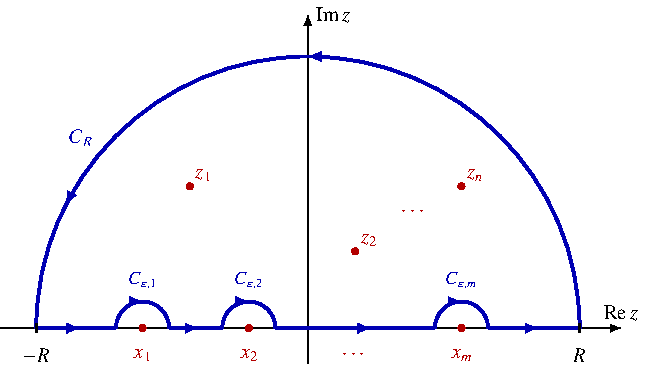
\includegraphics{papers/hauptwert/images/kontur-allgemein.pdf}
\caption{Der Integrationsweg $\Gamma$ im Beweis von
Satz~\ref{hauptwert:satz:hauptformel}, im positiven Sinn durchlaufen.
Auf der reellen Achse wird von $-R$ bis $R$ integriert, wobei um jede
Polstelle $x_j$ das Intervall $[x_j-\varepsilon, x_j+\varepsilon]$
ausgespart und durch die Einbuchtung $C_{\varepsilon,j}$ ersetzt wird.
Der grosse Halbkreis $C_R$ schliesst den Weg.
Die Einbuchtungen halten die Polstellen $x_1,\dots,x_m$ ausserhalb des
umlaufenen Gebietes, innerhalb liegen daher genau die Polstellen
$z_1,\dots,z_n$ der oberen Halbebene.
\label{hauptwert:figure:kontur-allgemein}}
\end{figure}


Dank der beiden Lemmata kann nun der Residuensatz auf Integrale über die
reelle Achse angewandt werden.
Das ermöglicht uns, uneigentliche Integrale mit dem Hauptwert zu berechnen.
Die Strategie ist dabei dieselbe wie im
Beispiel aus Abschnitt~\ref{hauptwert:subsection:aufwaermbeispiel}:
Die Strecke $[-R, R]$ wird durch den grossen Halbkreis
$C_R$ zu einem geschlossenen Weg ergänzt und die Polstellen auf der
Achse werden durch kleine Kreisbogen umgangen
(Abbildung~\ref{hauptwert:figure:kontur-allgemein}).

Damit der Residuensatz funktioniert, muss der Integrand vier Bedingungen
erfüllen.

\begin{satz}[Hauptwertformel]
\label{hauptwert:satz:hauptformel}
Die Funktion $f$ erfülle die folgenden Voraussetzungen:
\begin{enumerate}
  \item $f$ ist in der oberen Halbebene holomorph, also überall komplex
  differenzierbar, bis auf endlich viele isolierte Singularitäten.
  \item Auf der reellen Achse hat $f$ höchstens Polstellen erster Ordnung
  $x_1,\dots,x_m$.
  \item In der offenen oberen Halbebene hat $f$ keine anderen Singularitäten
  als die Polstellen $z_1,\dots,z_n$.
  \item Auf dem grossen Halbkreis $C_R$ fällt $f$ schneller als $1/|z|$,
  es gilt also
  \begin{equation}
    \max_{z \in C_R} |z\,f(z)| \to 0
    \qquad (R \to \infty).
    \label{hauptwert:equation:abfallbedingung}
  \end{equation}
\end{enumerate}
Dann gilt
\begin{equation}
  \pv \int_{-\infty}^{\infty} f(x)\,dx
  =
  2i\pi \sum_{k=1}^{n} \res(z_k; f)
  +
  i\pi \sum_{j=1}^{m} \res(x_j; f).
  \label{hauptwert:equation:hauptformel}
\end{equation}
\end{satz}

\begin{proof}
  Es wird entlang des Weges $\Gamma$ integriert
  (Abbildung~\ref{hauptwert:figure:kontur-allgemein}). Dieser setzt sich
  aus verschiedenen Teilen zusammen und wird im positiven Sinn
  (d.h. im Gegenuhrzeigersinn) durchlaufen. Auf der reellen Achse
  wird von $-R$ bis $R$ integriert, wobei um jede Polstelle $x_j$
  das Intervall $[x_j - \varepsilon, x_j + \varepsilon]$ ausgespart und
  durch den kleinen Halbkreisbogen $C_{\varepsilon,j}$ mit Radius
  $\varepsilon$ ersetzt wird. $\varepsilon$ wird so klein
  gewählt, dass keine kleinen Kreisbogen sich mit anderen
  Polstellen überschneiden.
  Geschlossen wird der Weg mit dem grossen Halbkreis $C_R$, welcher
  in der oberen Halbebene von $R$ zurück nach $-R$ verläuft. Der
  Radius $R$ wird so gross gewählt, dass alle Singularitäten in
  dieser oberen Halbebene innerhalb von $\Gamma$ liegen.
  Die Einbuchtungen schliessen die Polstellen $x_1, \dots, x_m$ aus dem
  umlaufenen Gebiet aus.
  Innerhalb von $\Gamma$ liegen daher genau die Polstellen
  $z_1, \dots, z_n$.

  Wäre $f$ im umlaufenen Gebiet überall holomorph, dann wäre das
  Wegintegral nach
  Satz~\ref{buch:integration:wegintegral:satz:zusammenziehbar} gleich $0$.
  Innerhalb von $\Gamma$ liegen aber die Polstellen $z_1, \dots, z_n$, und
  nach \eqref{buch:analytisch:laurentreihen:residuum:eqn:integralres} wird
  das Wegintegral allein durch deren Residuen bestimmt,
  \begin{equation}
    \oint_{\Gamma} f(z)\,dz
    =
    2i\pi \sum_{k=1}^{n} \res(z_k;f).
    \label{hauptwert:equation:gamma-residuen}
  \end{equation}

  Derselbe Weg lässt sich andererseits in seine Bestandteile zerlegen.
  Für die Streckenstücke auf der reellen Achse, aus denen die Intervalle
  $[x_j-\varepsilon, x_j+\varepsilon]$ ausgespart sind, wird zur Abkürzung
  \begin{equation}
    S(\varepsilon, R)
    =
    \int_{-R}^{x_1-\varepsilon} f(x)\,dx
    +
    \sum_{j=1}^{m-1} \int_{x_j+\varepsilon}^{x_{j+1}-\varepsilon} f(x)\,dx
    +
    \int_{x_m+\varepsilon}^{R} f(x)\,dx
    \label{hauptwert:equation:strecken}
  \end{equation}
  geschrieben.
  Alle Einbuchtungen haben denselben Radius $\varepsilon$ und die äusseren
  Grenzen sind symmetrisch, $S(\varepsilon,R)$ ist also genau die
  symmetrische Annäherung aus
  Definition~\ref{hauptwert:definition:pol}, übertragen auf $m$ Polstellen.
  Zusammen mit den Einbuchtungen und dem grossen Halbkreis ist
  \begin{equation}
    \oint_{\Gamma} f(z)\,dz
    =
    S(\varepsilon, R)
    +
    \sum_{j=1}^{m} \int_{C_{\varepsilon,j}} f(z)\,dz
    +
    \int_{C_R} f(z)\,dz.
    \label{hauptwert:equation:zerlegung}
  \end{equation}

  Die drei Summanden werden nun einzeln für $\varepsilon \to 0^+$ und
  $R \to \infty$ untersucht.
  Nach der zweiten Voraussetzung hat $f$ in jeder Stelle $x_j$ eine
  Polstelle erster Ordnung, auf jede Einbuchtung lässt sich also
  Lemma~\ref{hauptwert:lemma:halbresiduen} anwenden, und zusammen ergeben
  sie
  \begin{equation}
    \lim_{\varepsilon \to 0^+} \sum_{j=1}^{m} \int_{C_{\varepsilon,j}} f(z)\,dz
    =
    -i\pi \sum_{j=1}^{m} \res(x_j;f).
    \label{hauptwert:equation:einbuchtungen}
  \end{equation}
  Der grosse Halbkreis hat die Länge $\pi R$, und auf ihm ist $|z| = R$.
  Mit der Abfallbedingung \eqref{hauptwert:equation:abfallbedingung}
  verschwindet sein Beitrag daher,
  \begin{equation}
    \biggl| \int_{C_R} f(z)\,dz \biggr|
    \le
    \pi R \max_{z \in C_R} |f(z)|
    =
    \pi \max_{z \in C_R} |z\,f(z)|
    \to 0
    \qquad (R \to \infty).
    \label{hauptwert:equation:grosserbogen}
  \end{equation}

  Die linke Seite von \eqref{hauptwert:equation:zerlegung} hängt weder von
  $\varepsilon$ noch von $R$ ab, und die beiden letzten Summanden besitzen
  nach \eqref{hauptwert:equation:einbuchtungen} und
  \eqref{hauptwert:equation:grosserbogen} je einen Grenzwert.
  Also besitzt auch $S(\varepsilon,R)$ einen Grenzwert, und dieser ist nach
  Definition~\ref{hauptwert:definition:pol} der Hauptwert
  $\pv \int_{-\infty}^{\infty} f(x)\,dx$.
  Der Grenzübergang in \eqref{hauptwert:equation:zerlegung} liefert mit
  \eqref{hauptwert:equation:gamma-residuen} somit
  \begin{equation}
    \begin{aligned}
      \pv \int_{-\infty}^{\infty} f(x)\,dx
      - i\pi \sum_{j=1}^{m} \res(x_j;f)
      &=
      2i\pi \sum_{k=1}^{n} \res(z_k;f)
      \\
      \pv \int_{-\infty}^{\infty} f(x)\,dx
      &=
      2i\pi \sum_{k=1}^{n} \res(z_k;f)
      +
      i\pi \sum_{j=1}^{m} \res(x_j;f).
    \end{aligned}
  \end{equation}

  Damit ist auch die Frage beantwortet, die die Rechnung
  \eqref{hauptwert:equation:unsymmetrisch} offen gelassen hat.
  Jede Einbuchtung hat links und rechts denselben Radius $\varepsilon$, die
  Kontur nähert sich der Polstelle also von beiden Seiten gleich schnell.
  Die symmetrische Annäherung ist hier keine Konvention mehr, sondern eine
  Eigenschaft des Integrationsweges, und
  \eqref{hauptwert:equation:einbuchtungen} zeigt, was sie kostet, nämlich
  $-i\pi\res(x_j;f)$ für jede Polstelle auf der Achse.
\end{proof}


\subsection{Ein Warnbeispiel -- Was passiert, wenn die vierte Voraussetzung
nicht erfüllt ist?
\label{hauptwert:subsection:warnbeispiel}}

Das Integral
\begin{equation}
  \int_{-\infty}^{\infty} \frac{x + 1}{1 + x^2}\,dx
\end{equation}
haben wir in Abschnitt~\ref{hauptwert:subsection:weiteres-beispiel} bereits
mit dem reellen Hauptwert erfolgreich gelöst.
Wenn man hier jedoch den komplexen Weg mit der Halbkreiskontur geht,
entdeckt man, dass die vierte Voraussetzung nicht erfüllt ist.
Mit $f(z) = \frac{z + 1}{1 + z^2}$ ist
\begin{equation}
  |z\,f(z)|
  =
  \biggl| \frac{z(z + 1)}{1 + z^2} \biggr|
  \to
  1
  \qquad (|z| \to \infty),
  \label{hauptwert:equation:warnbeispiel-abfall}
\end{equation}
der Integrand fällt also genau wie $1/|z|$ und damit zu langsam.
Satz~\ref{hauptwert:satz:hauptformel} ist auf $f$ nicht anwendbar.

Die übrigen Voraussetzungen sind dagegen erfüllt.
Auf der reellen Achse hat $f$ keine Polstelle, und in der oberen Halbebene
liegt mit $z_1 = i$ genau eine.
Der rechten Seite von \eqref{hauptwert:equation:hauptformel} sieht man die
fehlende Voraussetzung nicht an, sie lässt sich ohne weiteres ausrechnen.
Das Residuum in $z_1$ ist
\begin{equation}
  \res(z_1;f)
  =
  \biggl.\frac{z + 1}{(1 + z^2)'}\biggr|_{z = i}
  =
  \frac{i + 1}{2i}
  =
  \frac{(i + 1)(-i)}{2i \cdot (-i)}
  =
  \frac{1 - i}{2},
  \label{hauptwert:equation:warnbeispiel-residuum}
\end{equation}
und die Residuensumme wird damit
\begin{equation}
  2i\pi \res(z_1;f)
  =
  2i\pi \cdot \frac{1 - i}{2}
  =
  i\pi (1 - i)
  =
  \pi + i\pi .
  \label{hauptwert:equation:warnbeispiel-falsch}
\end{equation}
Diese Zahl ist nicht reell, sie kann also nicht der Hauptwert des Integrals
einer reellen Funktion sein.
Der Vergleich mit
Abschnitt~\ref{hauptwert:subsection:weiteres-beispiel} bestätigt es:
Dort ergab dasselbe Integral den Wert $\pi$.

Verantwortlich dafür ist der grosse Halbkreis.
Die Abschätzung \eqref{hauptwert:equation:grosserbogen} aus dem Beweis
liefert wegen \eqref{hauptwert:equation:warnbeispiel-abfall} nur noch die
Schranke $\pi$ statt $0$, sein Beitrag muss also nicht mehr verschwinden.
Wie gross er ist, lässt sich ohne weitere Rechnung ablesen.
Da $f$ auf der reellen Achse keine Polstelle hat, besteht der geschlossene
Weg nur aus der Strecke und dem Bogen, und der Residuensatz liefert für
jedes $R > 1$
\begin{equation}
  \int_{-R}^{R} f(x)\,dx
  +
  \int_{C_R} f(z)\,dz
  =
  \pi + i\pi .
  \label{hauptwert:equation:warnbeispiel-bilanz}
\end{equation}
Das erste Integral geht nach
Abschnitt~\ref{hauptwert:subsection:weiteres-beispiel} gegen $\pi$, für den
Bogen bleibt also
\begin{equation}
  \lim_{R \to \infty} \int_{C_R} f(z)\,dz
  =
  \pi + i\pi - \pi
  =
  i\pi
  \neq
  0 .
  \label{hauptwert:equation:warnbeispiel-bogen}
\end{equation}
Genau um diesen Term liegt die Residuensumme neben dem Hauptwert.

Gefährlich ist dabei, dass die Rechnung trotz fehlender Voraussetzung zu
funktionieren scheint:
Es divergiert nichts, und trotzdem ist das Resultat falsch.


\subsection{Das Dirichlet-Integral
\label{hauptwert:subsection:dirichlet}}

Zum Abschluss eine Anwendung, die mit reellen Mitteln nur mühsam zugänglich
ist, weil der Integrand keine elementare Stammfunktion hat.
Gesucht ist der Wert des \emph{Dirichlet-Integrals}
\begin{equation}
  \int_{0}^{\infty} \frac{\sin x}{x}\,dx .
  \label{hauptwert:equation:dirichlet}
\end{equation}

Da sich der Integrand bei $x = 0$ stetig ergänzen lässt, liegt gar keine
Polstelle auf der reellen Achse vor.
Die Polstelle entsteht erst durch den Übergang ins Komplexe.
Betrachtet wird die Funktion
\begin{equation}
  f(z) = \frac{e^{iz}}{z}.
\end{equation}
Teilt man sie auf der reellen Achse in Kosinus und Sinus auf, so wird
sichtbar, woher die Polstelle kommt,
\begin{equation}
  \frac{e^{ix}}{x} = \frac{\cos x}{x} + i\,\frac{\sin x}{x} .
  \label{hauptwert:equation:dirichlet-zerlegen}
\end{equation}
Der Sinusanteil ist der gesuchte Integrand und in $x = 0$ stetig ergänzbar,
der Kosinusanteil dagegen nicht.
Er trägt die Singularität, und $f$ hat in $x_1 = 0$ eine Polstelle erster
Ordnung.

Satz~\ref{hauptwert:satz:hauptformel} ist auf $f$ nicht direkt anwendbar.
Auf dem grossen Halbkreis ist $|z\,f(z)| = |e^{iz}| = e^{-R\sin\theta}$, was
an den Endpunkten $\theta = 0$ und $\theta = \pi$ gleich $1$ ist, die
vierte Bedingung \eqref{hauptwert:equation:abfallbedingung} ist also verletzt.
Hier hilft uns das Lemma von Jordan.

Integriert wird über denselben Weg $\Gamma$ wie im Beweis von
Satz~\ref{hauptwert:satz:hauptformel}, mit einer einzigen Einbuchtung
$C_\varepsilon$ um $x_1 = 0$.
Weitere Singularitäten hat $f$ in der oberen Halbebene nicht und gemäss
Satz~\ref{buch:integration:wegintegral:satz:zusammenziehbar} verschwindet das
Wegintegral,
\begin{equation}
  \int_{-R}^{-\varepsilon} f(x)\,dx
  +
  \int_{\varepsilon}^{R} f(x)\,dx
  +
  \int_{C_\varepsilon} f(z)\,dz
  +
  \int_{C_R} f(z)\,dz
  =
  0 .
  \label{hauptwert:equation:dirichlet-zerlegung}
\end{equation}

Für die Einbuchtung ist das Residuum
\begin{equation}
  \res(x_1;f)
  =
  \lim_{z \to 0} z\,\frac{e^{iz}}{z}
  =
  1,
\end{equation}
nach Lemma~\ref{hauptwert:lemma:halbresiduen} trägt sie also
$-i\pi\res(x_1;f) = -i\pi$ bei.
Für den grossen Halbkreis ist $f(z) = g(z)e^{iaz}$ mit $g(z) = \frac{1}{z}$
und $a = 1$, und wegen $\max_{z \in C_R} |g(z)| = \frac{1}{R} \to 0$
verschwindet sein Beitrag nach Lemma~\ref{hauptwert:lemma:jordan}.
Aus \eqref{hauptwert:equation:dirichlet-zerlegung} wird damit
\begin{equation}
  \pv \int_{-\infty}^{\infty} \frac{e^{ix}}{x}\,dx
  -
  i\pi
  =
  0 .
  \label{hauptwert:equation:dirichlet-komplex}
\end{equation}

Der Realteil $\frac{\cos x}{x}$ aus
\eqref{hauptwert:equation:dirichlet-zerlegen} ist ungerade, seine Beiträge
heben sich bei symmetrischer Annäherung weg, und genau das spiegelt sich
darin, dass
\eqref{hauptwert:equation:dirichlet-komplex} rein imaginär ist.
Der Imaginärteil liefert
\begin{equation}
  \pv \int_{-\infty}^{\infty} \frac{\sin x}{x}\,dx = \pi .
\end{equation}
Hier ist der Hauptwert allerdings nicht mehr nötig, denn der Integrand ist in
$0$ stetig ergänzbar und gerade, es ist also
$\int_{-R}^{R} = 2\int_{0}^{R}$.
Der symmetrische Grenzwert ist damit das gewöhnliche uneigentliche Integral,
und für \eqref{hauptwert:equation:dirichlet} folgt
\begin{equation}
  \int_{0}^{\infty} \frac{\sin x}{x}\,dx = \frac{\pi}{2}.
\end{equation}

Bemerkenswert daran ist die Rolle, die der Hauptwert hier spielt.
Er rettet kein divergentes Integral, sondern ist ein Rechenwerkzeug.
Der gesuchte Integrand hat gar keine Polstelle, erst der Ersatz durch
$\frac{e^{iz}}{z}$ erzeugt eine, die dann durch den Hauptwert regularisiert
wird.
